\documentclass[12pt,fleqn]{article}\usepackage{../../common}
\begin{document}
Sonlu Hacim (Finite Volume) Yöntemi - 2

Amaç bir diferansiyel denklemi sayısal olarak çözmek. Metot olarak sonlu
farklılık (finite difference -FD-) yöntemi daha önce işlendi, bu yöntemde bir
sürekli fonksiyonun değerlerini ayrıksal noktalar üzerinden temsil etmeye
uğraşıyorduk.  Bu noktalar bir ekseni eşit aralıklara bölerek ortaya
çıkartılıyordu, mesela altta görülen bir tepeyle başlayıp inen $f$ fonksiyonu
$i-2,i-1,i,..$ noktalarında $x_i$ değerleri üzerinden $u_i = u(x_i)$ ile
tanımlanıyordu.

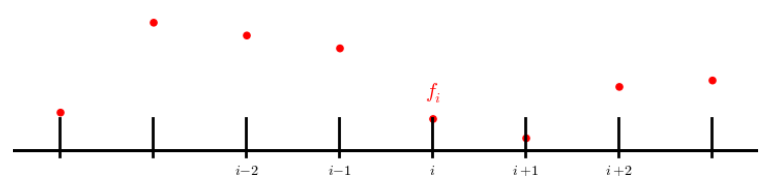
\includegraphics[width=30em]{13-22-29.png}

Sonlu hacim (FV) yönteminde durum biraz farklı; bir fonksiyonu belli
noktalarındaki noktasal değerlerle değil, belli aralıklar arasında kalan
değerlerinin {\em averajı} olarak temsil ediyoruz.

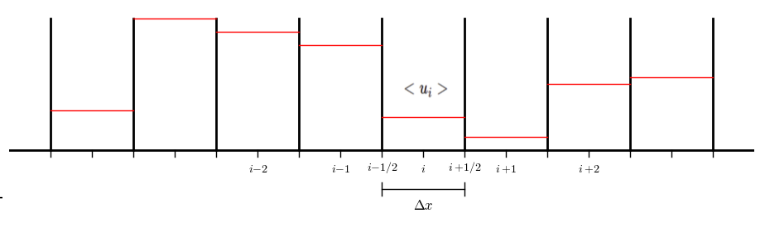
\includegraphics[width=30em]{13-22-34.png}

Farklı bir grafik

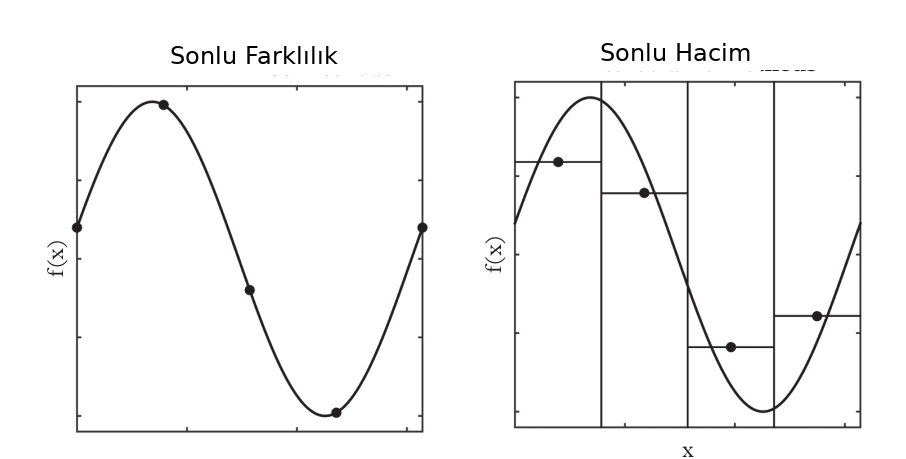
\includegraphics[width=30em]{13-16-00.png}

İki üstte görülen grafikte mesela $i$ ile $i+1$ noktası ortasındaki $i+1/2$
noktası ve $i$ ile $i-1$ noktası ortasındaki $i-1/2$ arasında kalan fonksiyonun
averajı alınacak, ona $< u_i >$ ya da $\overline{u}_i$ diyoruz.

$$
\overline{u}_i = \frac{1}{\Delta x} \int _{x_{i-1/2}}^{x_{i+1/2}} u(x) \ud x
$$

Dikkat; $i-1,i-2$ değerleri $i$ referanslı olduğu için eksi içerikli, $i=4$
olsaydı onlar $3,2,..$ diye gidebilirdi. Ayrıca FD yönteminin aksine, indis
değerlerine tekabül eden $x_i,x_{i+1}$ değerleri herhangi bir yerde olabilir,
böylece eşit aralıklı olmayan ızgaralarla çalışmamız mümkün olur, bu FV
yönteminin kuvvetlerinden biri. 

Gerçi biz bu anlatımda ve kodda eşit aralık farz edeceğiz, $\Delta x$, $h_x$
burada devreye girer. 

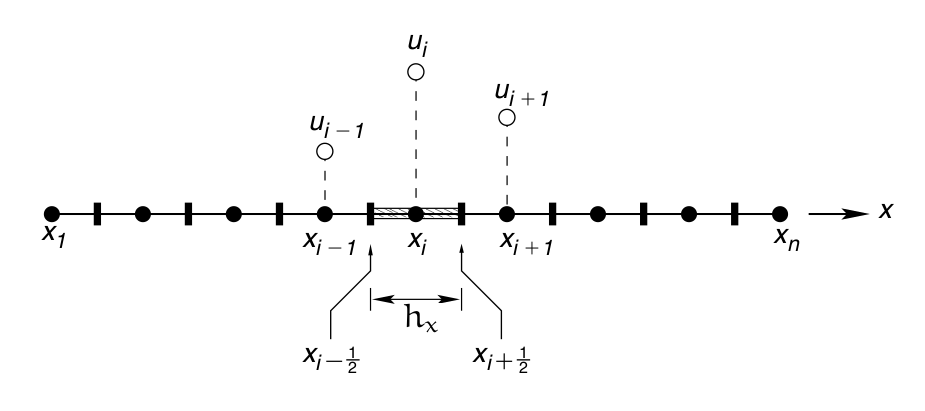
\includegraphics[width=20em]{12-20-00.png}

Muhafaza Kanunu Hesaplamak

Notasyonda $f$ akış (flux) için kullanılır [2], $\Delta x$ için $h_x$,

$$
\overline{u}_i =  \frac{1}{h_x} \int_{x_{i-1/2}}^{x_{i+1/2}} u(x) \ud x
\mlabel{1}
$$

[3] yazısında muhafaza kanununun entegral formunu görmüştük,

$$
\int _{x_1}^{x_2} \rho(x,t_2) \ud x =
\int _{x_1}^{x_2} \rho(x,t_1) \ud x  +
\int_{t_1}^{t_2} \rho(x_1,t) v(x_1,t) \ud t -
\int_{t_1}^{t_2}  \rho(x_2,t) v(x_2,t) \ud t
$$

$f(\rho) = \rho(x,t) v(x,t)$ denebilir, ya da herhangi daha genel olarak $\rho$
yerine herhangi bir ölçüm $u$ için $f(u) = u(x,t) v(x,t)$, o zaman, ve
biraz yer değişim sonrası,

$$
\int_{x_1}^{x_2} u(x,t_2) \ud x -
\int_{x_1}^{x_2} u(x,t_1) \ud x  +
\int_{t_1}^{t_2} f(x_2,t) \ud t  -
\int_{t_1}^{t_2} f(x_1,t) \ud t = 0
$$

Bu formülü her sonlu hacim hücresi için kullanacağız. Zaman indisleri $t,t+1$
olacak, üstte $t_1,t_2$ yerine. Yer için $x_1,x_2$ yerine bir $j$ indisi
merkezli $x_{j-1/2}$ ve $x_{j+1/2}$. Devam edelim, $u(x_1,t_1)$ içinde
$x_{j-1/2}$ ve $t_l$ oluyor, (zaman $l$ indisi) ona da $u_{j-1}^l$
diyelim. $x_2$ yerine $x_{j+1/2}$, sonuncuda zamanın hala değişken olduğu durum
$u_{j+1}$ olsun. Eğer $x$ değişken ise, zaman indisi $t_2 = t_{l+1}$ için
$u^{l}$. Üstteki formülü bu notasyonla değiştirip istenen zaman ve yer
aralıklarına uygularsak,

$$
\int_{x_{j-1/2}}^{x_{j+1/2}} u^{l+1} \ud x -
\int_{x_{j-1/2}}^{x_{j+1/2}} u^{l} \ud x  +
\int_{t_l}^{t_{l+1}} f(u_{j+1/2}) \ud t  -
\int_{t_l}^{t_{l+1}} f(u_{j-1/2}) \ud t = 0
$$

Her şeyi $h_x$ ile bölelim,

$$
\frac{1}{h_x} \int_{x_{j-1/2}}^{x_{j+1/2}} u^{l+1} \ud x -
\frac{1}{h_x} \int_{x_{j-1/2}}^{x_{j+1/2}} u^{l} \ud x  +
\frac{1}{h_x} \int_{t_l}^{t_{l+1}} f(u_{j+1/2}) \ud t  -
\frac{1}{h_x} \int_{t_l}^{t_{l+1}} f(u_{j-1/2}) \ud t = 0
$$

Bu formülde (1)'de tanımlanan ortalama formunu görüyoruz, kısaltma amaçlı
$\overline{u}_{j,l}$ notasyonu oralarda kullanabiliriz,

$$
\overline{u}_{j,l+1} - \overline{u}_{j,l} + 
\frac{1}{h_x} \int_{t_l}^{t_{l+1}} f(u_{j+1/2}) \ud t  -
\frac{1}{h_x} \int_{t_l}^{t_{l+1}} f(u_{j-1/2}) \ud t = 0
$$

Şimdi son iki terime dikkat edelim, bu iki entegral zaman üzerinden alınıyor,
fakat Riemann problemini hatırlarsak çözüm $u(x,t)$ sadece $x/t$ değişkeni
üzerinden düşünülebilir, ve eğer $x$ değişmiyorsa (ki öyle çünkü üstteki iki
entegral $t$ üzerinden, $x$ aynı) o zaman $\ud t$ üzerinden entegral yerine,
sabit $u$ ile bir ayrıksal $h_t$ çarpımı yeterlidir. Öyle ya sabit $u$ üzerinden
ve yine sabit / bilinen $t$ adımı $h_t$ üzerinden alan bir dikdörtgendir, bu
alanın hesabı için çetrefil entegral yerine direk çarpım yeterli.. Mesela ilk
entegral,

$$
\frac{1}{h_x} \int_{t_l}^{t_{l+1}} f(u_{j+1/2}) \ud t =
\frac{h_t}{h_x} f(u_{j+1/2})
$$

olarak hesaplanabilir, çünkü $u$ değeri $x = x_{j \pm 1/2}$ üzerinde değişmiyor.
Aynı durum ikinci entegral için de geçerli, o zaman iki üstteki formül

$$
\overline{u}_{j,l+1} = \overline{u}_{j,l} -
\frac{h_t}{h_x} ( f(u_{j+1/2}) - f(u_{j-1/2}) )
\mlabel{2}
$$

olacak. Böylece $l$ anındaki $j$ hücresinin ortalamasını bir sonraki zaman adımı
$l+1$'e nasıl aktaracağımızı, oraya geçiş yapacağımızın formülünü bulmuş olduk.

Eğer $\frac{1}{h_x} \int_{t_l}^{t_{l+1}} f(u_{j+1/2}) \ud t$ entegralini
entegral içindekiler çarpı $h_t$ ile gösterebiliyorsak, tüm
entegrali $h_t$ ile bölmek bize yaklaşık, ``sayısal'' bir $f(u_{j+1/2})$
verecektir, ona büyük harf ile $F_{j+1/2}^l$ diyelim, formülü [4, sf. 103]

$$
F_{j+1/2}^l = \frac{1}{h_t} \int_{t_l}^{t_{l+1}} f(u_{j+1/2,l}) \ud t
$$

$F$'ye sayısal akış (numerical flux) ismi de veriliyor. O zaman (2) formülü
``akış diferansiyel formunda'' da yazılabilir,

$$
\overline{u}_{j,l+1} = \overline{u}_{j,l} -
\frac{h_t}{h_x} ( F_{j+1/2,l} - F_{j-1/2,l} )
$$

Sayısal akışı elde etmek için bize bir sayısal $u$ lazım, bunu FV ile bulacağız,
sonra bu $u$'ları bildiğimiz $f()$ akışına verince sayısal $F$ elde edilecek.

Bu kod alttaki gibidir,

\begin{minted}[fontsize=\footnotesize]{python}
import scipy.integrate as integrate
import matplotlib.pyplot as plt
import numpy as np

alpha = 0.0
beta  = 1.0

def init(z, alpha, beta):
    return alpha + beta*np.sin(z)

# 
#  u_t + f(u)_x = 0 denklemi icin akis (flux) fonksiyonu 
#
def flux(u):
    return 0.5*u**2

def godunov_flux(uval):
    fhat = np.zeros((len(uval),1))

    for i in range(0,len(uval)-1):
        ul = uval[i]; ur = uval[i+1]

        s=(ul+ur)/2;
        if ul > ur:
            if s < 0:
                fhat[i] = flux(ur)
            else:
                fhat[i] = flux(ul)
        elif ul < ur:
            if ur < 0:
                fhat[i] = flux(ur)
            elif ul > 0.:
                fhat[i] = flux(ul)
            else:
                fhat[i] = 0
                
    return fhat

a = 0
b = 2*np.pi
N  = 80
T = 2.0

x = np.linspace(a,b,N)     
dx = (b-a)/(N-1);  
u = np.zeros((len(x)-1,1)); 

for i in range(0,N-1):
    u[i] = (1.0/dx)*integrate.quad(init, x[i], x[i+1], args=(alpha,beta))[0]

dt = dx/(2*np.amax(np.amax(u)))

t = 0.0
i = 0
while t < T:
    fR = godunov_flux(u) 
    fL = np.roll(fR,1)
    u -= dt/dx*(fR - fL)
    t = t+dt
    i += 1

    if i % 5 == 0:
        plt.figure()
        plt.plot(u)
        plt.ylim(-1,1)
        plt.savefig('/tmp/out-%03d.png' % i)
        plt.close('all')
\end{minted}

Kodda ilk önce başlangıç fonksiyonu tanımlandı, içinde sinüs olan \verb!init!
bu; Bu fonksiyonun hücre bazında \verb!integrate.quad! ile entegrali alındı,
böylece her hücreyi temsil eden o tek değeri elde ettik.

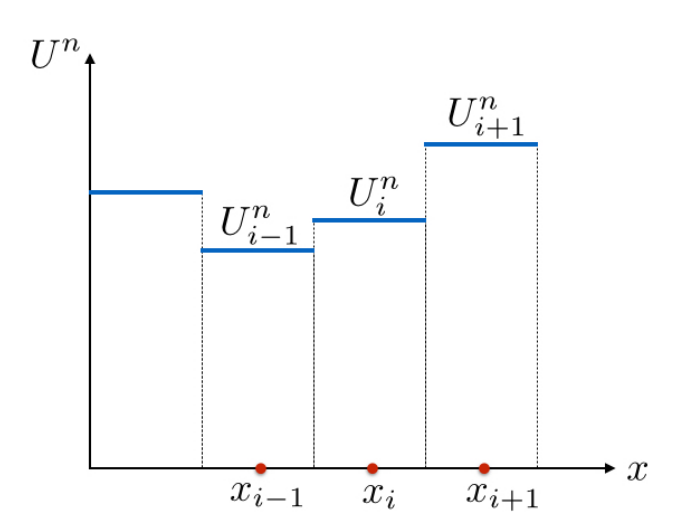
\includegraphics[width=12em]{12-19-02.png}

FV yöntemi bundan sonra o hücreler üzerinden hesabını yapacak, dinamik denklemi
zamanda ilerletirken bunun hücrelerdeki o temsili değer üzerinden yapacak.

Hücrelerin FV matematiği şöyle; mesela yanyana iki hücreye bakarsak, üstteki
resimde $x_{i-2}$ ve $x_{i-1}$ diyelim, soldan ilk iki hücre, bu iki değer sanki
bir Riemann problemini andırmıyor mu? Evet; ve Godunov'un icat ettiği FV çözümü
için kullanılan teknik te zaten budur. İki hücre ortasındaki $x_{i-1/2}$ noktası
hücre sınırı kabul edilir ve önceki sonraki değerler $u_L$ ve $u_R$ imiş gibi
Riemann çözümü işletilir. Bu işlem tüm yanyana hücreler için işletilince bir
zaman dilimi çözümü elde edilir, sonraki zaman dilimi için bu işlem tekrar
baştan hesaplanır.

Şimdi $x_{i}$ ile $x_{i+1}$ arasındaki $x_{1+1/2}$ sınırını baz alıp, ve
[3]'teki Riemann çözümünü baz alarak şunu yazalım [4, sf. 109],

$u_i^l \ge u_{i+1}^l$ için,

$$
u^\star_{i+1/2} = 
\left\{ \begin{array}{lll}
u_i^l & \textrm{eğer} & s > (x-x_{i+1/2}) / t  \\
u_{i+1}^l & \textrm{eğer} & s < (x-x_{i+1/2}) / t
\end{array} \right.
$$

Daha önce gördük $s$ dalga hızı, bu örnekte $s = (u_i^n + u_{i+1}^n)/2$.

$u_i^l < u_{i+1}^l$ için,

$$
u^\star_{i+1/2} = 
\left\{ \begin{array}{lll}
u_i^l & \textrm{eğer} & (x-x_{i+1/2})/t \le u_i^l   \\
(x-x_{i+1/2})/t & \textrm{eğer} & u_i^l < (x-x_{i+1/2})/t < u_{i+1}^l   \\
u_{i+1}^l & \textrm{eğer} & (x-x_{i+1/2})/t \ge u_{i+1}^l   \\
\end{array} \right.
$$

Bir kez Riemann çözümü elde edilince Godunov sayısal akışı $u^\star_{i+1/2}$ ile
kolayca hesaplanabilir, akış fonksiyonu $f()$ üzerinden $F = f(u^\star_{i+1/2})$.

Üstteki formülleri daha da kolaylaştırmak mümkün, Godunov akışlarını
$x = x_{i+1/2}$ noktasında hesapladığımız için bunu formülde $x$ yerine
koyunca,

$u_i^l \ge u_{i+1}^l$ için,

$$
u^\star_{i+1/2} = 
\left\{ \begin{array}{lll}
u_i^l & \textrm{eğer} & s > 0  \\
u_{i+1}^l & \textrm{eğer} & s < 0
\end{array} \right.
$$

$u_i^l < u_{i+1}^l$ için,

$$
u^\star_{i+1/2} = 
\left\{ \begin{array}{lll}
u_i^l & \textrm{eğer} & 0 \le u_i^l   \\
(x-x_{i+1/2})/t & \textrm{eğer} & u_i^l < 0 < u_{i+1}^l   \\
u_{i+1}^l & \textrm{eğer} & 0 \ge u_{i+1}^l   \\
\end{array} \right.
$$

Kod içinde üstte görülen hesabı tüm hücreler için yaptık, $i$,$i+1$,$i+2$.. ve
$F_{j+1/2,l}$ hesabından bir önceki $F_{j-1/2,l}$, kod içinde önceki \verb!fL!
sonraki \verb!fR!, onun için \verb!np.roll! ile vektör içindeki değerleri bir
ilerleterek önceki ve sonraki hücrelerin aynı hizaya düşmesini sağlıyoruz
böylece $F_{j+1/2,l}-F_{j-1/2,l}$ hesabı kolay bir şekilde \verb!fR-fL!
ile bulunabiliyor.

Belli $t$ anlarından alınmış görüntüler altta bulunabilir.

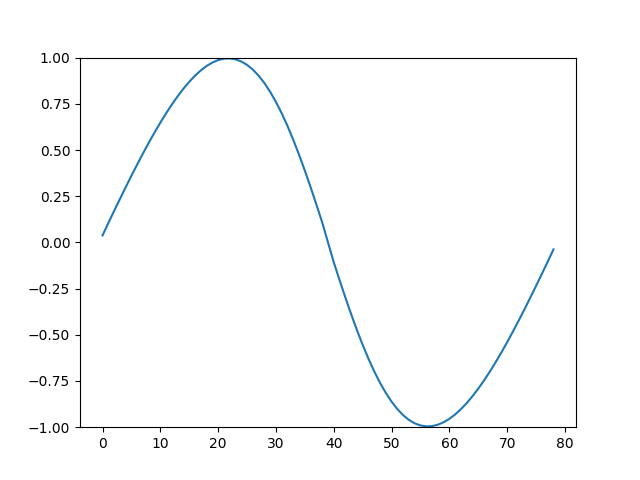
\includegraphics[width=20em]{out-005.png}
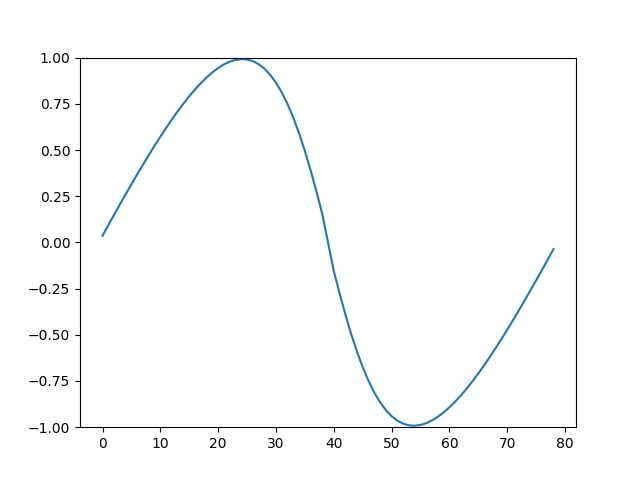
\includegraphics[width=20em]{out-010.png}
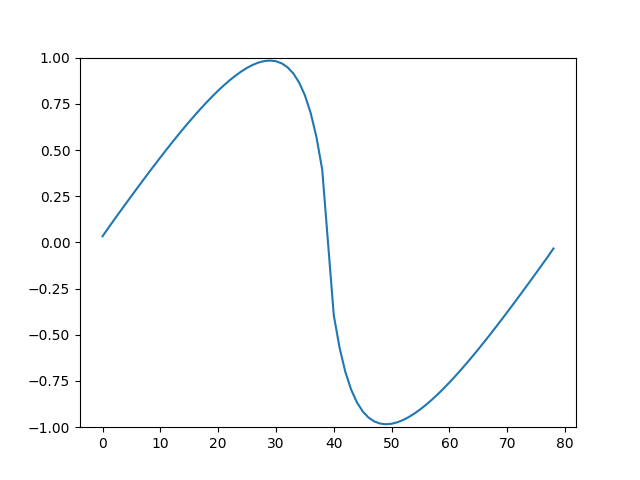
\includegraphics[width=20em]{out-020.png}
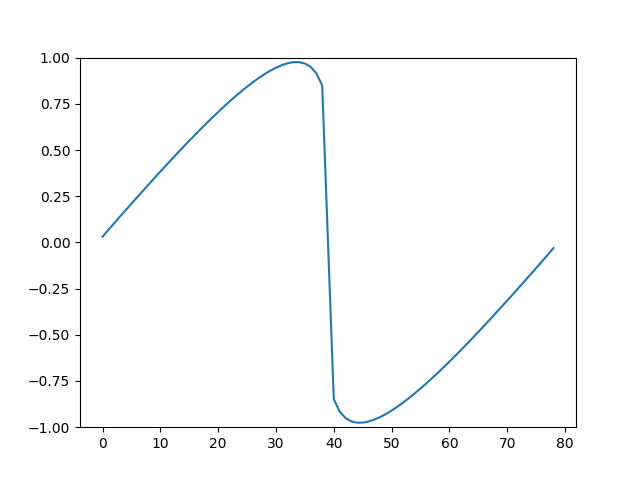
\includegraphics[width=20em]{out-030.png}

Animasyon [1],

\begin{minted}[fontsize=\footnotesize]{python}
! convert -delay 20 -loop 0 /tmp/out-*.png wave.gif
\end{minted}
  
Kaynaklar

[1] Bayramlı, {\em Animasyon, Godunov Sonlu Hacim Yontemi ile Burgers Denklem Cozumu}
    \url{https://github.com/burakbayramli/classnotes/raw/master/compscieng/compscieng_bpp50fv2/wave.gif}

[2] Kloeckner, {\em Numerical Methods for Partial Differential Equations CS555 / MATH555 / CSE510}
    \url{https://relate.cs.illinois.edu/course/cs555-s20/}

[3] Bayramlı, {\em Sonlu Hacim (Finite Volume) Yöntemi - 1}

[4] Lee, Computational Fluid Dynamics

\end{document}




